\documentclass{article}
\usepackage[UTF8]{ctex}
\usepackage{geometry}
\usepackage{makecell}
\usepackage{amsmath}
\usepackage{graphicx}
\usepackage{subcaption}

\geometry{a4paper,scale=0.75}

\title{\heiti 实验二十\ 光衍射的定量研究}
\author{\kaishu 田睿轩\ 物理学院\ 1900011602}
\date{2020年11月6日}
\newcommand{\degree}{^\circ}

\begin{document}
    \maketitle

    \section{实验内容与数据处理}
    
    \subsection{组装、调试光路}
    调整激光器高度和倾角,使激光器的光线平行于台面。通过观察激光器距离光屏不同距离时,
    光屏上光点的位置,可以确定激光是否平行于台面。

    调整反射镜的角度,使经反射后的光线平行于台面。在探测器上放一个反射镜,反射回来的
    光线应反射到激光器出口。通过观察反射回来的激光光点位置调整反射镜角度。

    调整衍射屏的位置,使狭缝垂直于台面。通过观察衍射条纹在光屏上是否水平可以确定衍射屏
    是否垂直于台面。

    调整衍射屏的角度,使激光垂直于狭缝入射。由于衍射屏狭缝周围是镜面,所以若是垂直入射,
    激光会被反射回反射镜,在激光器出口形成亮纹,可以据此来判断激光是否垂直入射。

    另外,为了保证夫琅和费衍射的远场接收条件,衍射屏与探测器的距离要足够远。

    \subsection{测量单缝衍射条纹光强曲线并计算缝宽}
    使用探测器进行扫描,记录衍射不同位置的光强并绘制曲线。扫描过程中以$0.005mm$为间隔
    进行扫描,扫描范围为$20cm$,得到如下扫描曲线:

    \vspace{2ex}
    \includegraphics[scale=0.44]{single.jpg}

    根据夫琅和费衍射公式,衍射条纹的光强满足:
    $$I_\theta = I_0(\frac{\sin \alpha}{\alpha})^2$$
    
    主极强到第一次极强的衍射角度$\theta$满足
    $$\sin \theta=1.43\frac{\lambda}{b}=\frac{\Delta x}{Z}$$
    其中$b$为狭缝宽度,$\Delta x$为主极强到第一次极强的距离,$Z$为衍射屏到探测器探头距离。
    
    在曲线中读出主极强和两个第一次极强的位置及光强:
    
    %\vspace{1ex}
    \begin{center}
        \begin{tabular}{|c|c|c|c|}
            \hline
            物理量 & 主极强 & 左侧第一次极强 & 右侧第一次极强 \\
            \hline
            相对光强 & 3985 & 181 & 175 \\
            \hline
            绝对坐标($cm$) & 11.130 & 7.620 & 14.650\\
            \hline
        \end{tabular}
    \end{center}
    %\vspace{1ex}

    计算两次极强光强对称比和次极强与主极强之间的峰值比:
    $$\frac{I_1-I_2}{\frac{I_1+I_2}{2}}=1.1\% $$
    $$\frac{I_1+I_2}{2I_0}=4.5\%$$
    
    衍射条纹的对称度较好,说明基本满足了衍射屏垂直于台面,激光基本垂直于衍射屏入射,
    且衍射屏基本垂直于台面

    实验中,衍射屏的位置为$24.8cm$,探测器底座边缘为$93.8cm$,探测器探头到底座边缘距离
    为$0.4cm$,故衍射屏到探测器探头距离$Z=93.8-24.8+0.4=69.4cm$

    主极强到两次极强的平均距离$\Delta x = \frac{x_2-x_1}{2}=3.515mm$

    实验中,使用的是波长$\lambda=632.8nm$的He-Ne激光,代入数据,可得
    $$b=1.43\frac{\lambda Z}{\Delta x}=178.1\mu m$$

    \subsection{测量三缝衍射条纹光强曲线和缝宽、缝间距}
    更换衍射屏,重新调整其位置和水平、竖直,使用探测器进行扫描,记录衍射不同位置的光强并绘制曲线。扫描过程中以$0.005mm$为间隔
    进行扫描,扫描范围为$20cm$,得到如下扫描曲线:

    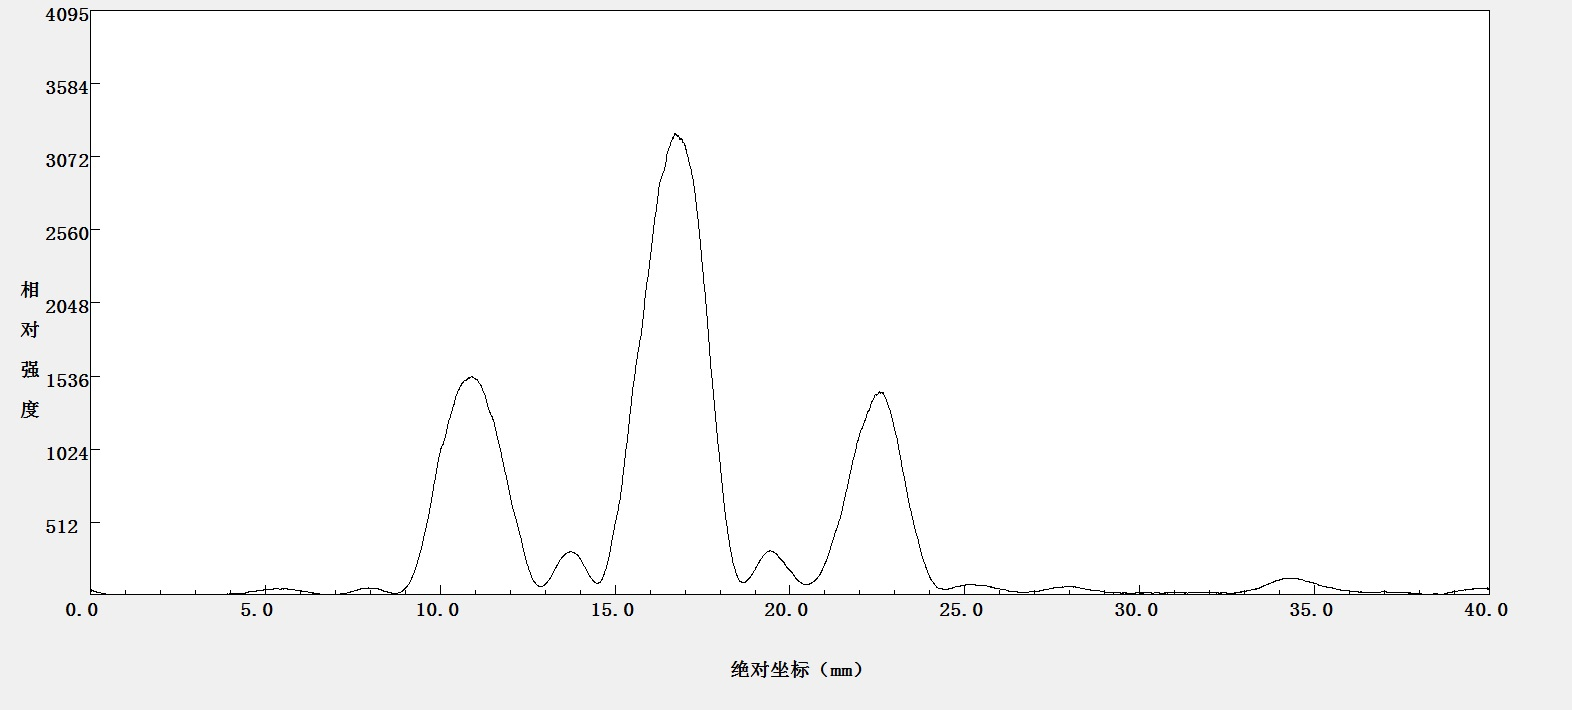
\includegraphics[scale=0.44]{trible.jpg}
    \vspace{2ex}

    多缝夫琅禾费衍射满足公式:
    $$I_\theta = I_0 (\frac{\sin \alpha}{\alpha})^2 (\frac{\sin N\beta}{\sin \beta})^2$$
    其中:$(\frac{\sin \alpha}{\alpha})^2$为单缝衍射因子,决定了光强曲线包络线的形状,
    $(\frac{\sin N\beta}{\sin \beta})^2$为多缝干涉因子,使得光强曲线在几个主极强之间出现次极强和暗纹

    根据单缝衍射因子可以求出缝宽$b$:
    $$\sin \theta = \frac{\lambda}{b} = \frac{\Delta x}{Z}$$
    其中$\Delta x $为包络线上中央主极强到第一暗纹的距离

    通过局部寻峰和局部寻谷,得出中央主极强和包络线第一暗纹的坐标:

    %\vspace{1ex}
    \begin{center}
        \begin{tabular}{|c|c|c|c|}
            \hline
            物理量 & 主极强 & 左侧第一暗纹 & 右侧第一暗纹 \\
            \hline
            绝对坐标($cm$) & 16.710 & 2.370 & 29.690\\
            \hline
        \end{tabular}
    \end{center}
    %\vspace{1ex}

    实验中,衍射屏位置为$9.6cm$,探测器底部位置为$93.8cm$,故衍射屏到探测器探头距离
    为$Z=93.8-9.6+0.4=84.6cm$

    主极强到第一暗纹的距离$\Delta x =\frac{x_2-x_1}{2}=13.66mm$

    带入衍射公式,得:
    $$b=\frac{\lambda Z}{\Delta x}=39.1\mu m$$

    根据多缝干涉因子可以求出缝宽$d$:
    $$\sin \theta = \frac{\lambda}{d} = \frac{\Delta x^{'}}{Z}$$
    其中$\Delta x^{'}$为光强曲线上中央主极强到第一暗纹的距离
    
    通过局部寻峰和局部寻谷,得出中央主极强和第一暗纹的坐标:

    %\vspace{1ex}
    \begin{center}
        \begin{tabular}{|c|c|c|c|}
            \hline
            物理量 & 主极强 & 左侧第一暗纹 & 右侧第一暗纹 \\
            \hline
            绝对坐标($cm$) & 16.710 & 10.90 & 22.55\\
            \hline
        \end{tabular}
    \end{center}
    %\vspace{1ex}

    主极强到第一暗纹的距离$\Delta x^{'} =\frac{x_2-x_1}{2}=5.825mm$

    带入衍射公式,得:
    $$d=\frac{\lambda Z}{\Delta x^{'}}=91.8\mu m$$

    \subsection{其他衍射结构的衍射图样}    
    \begin{figure*}
        \centering
        \begin{subfigure}[b]{0.45\textwidth}
            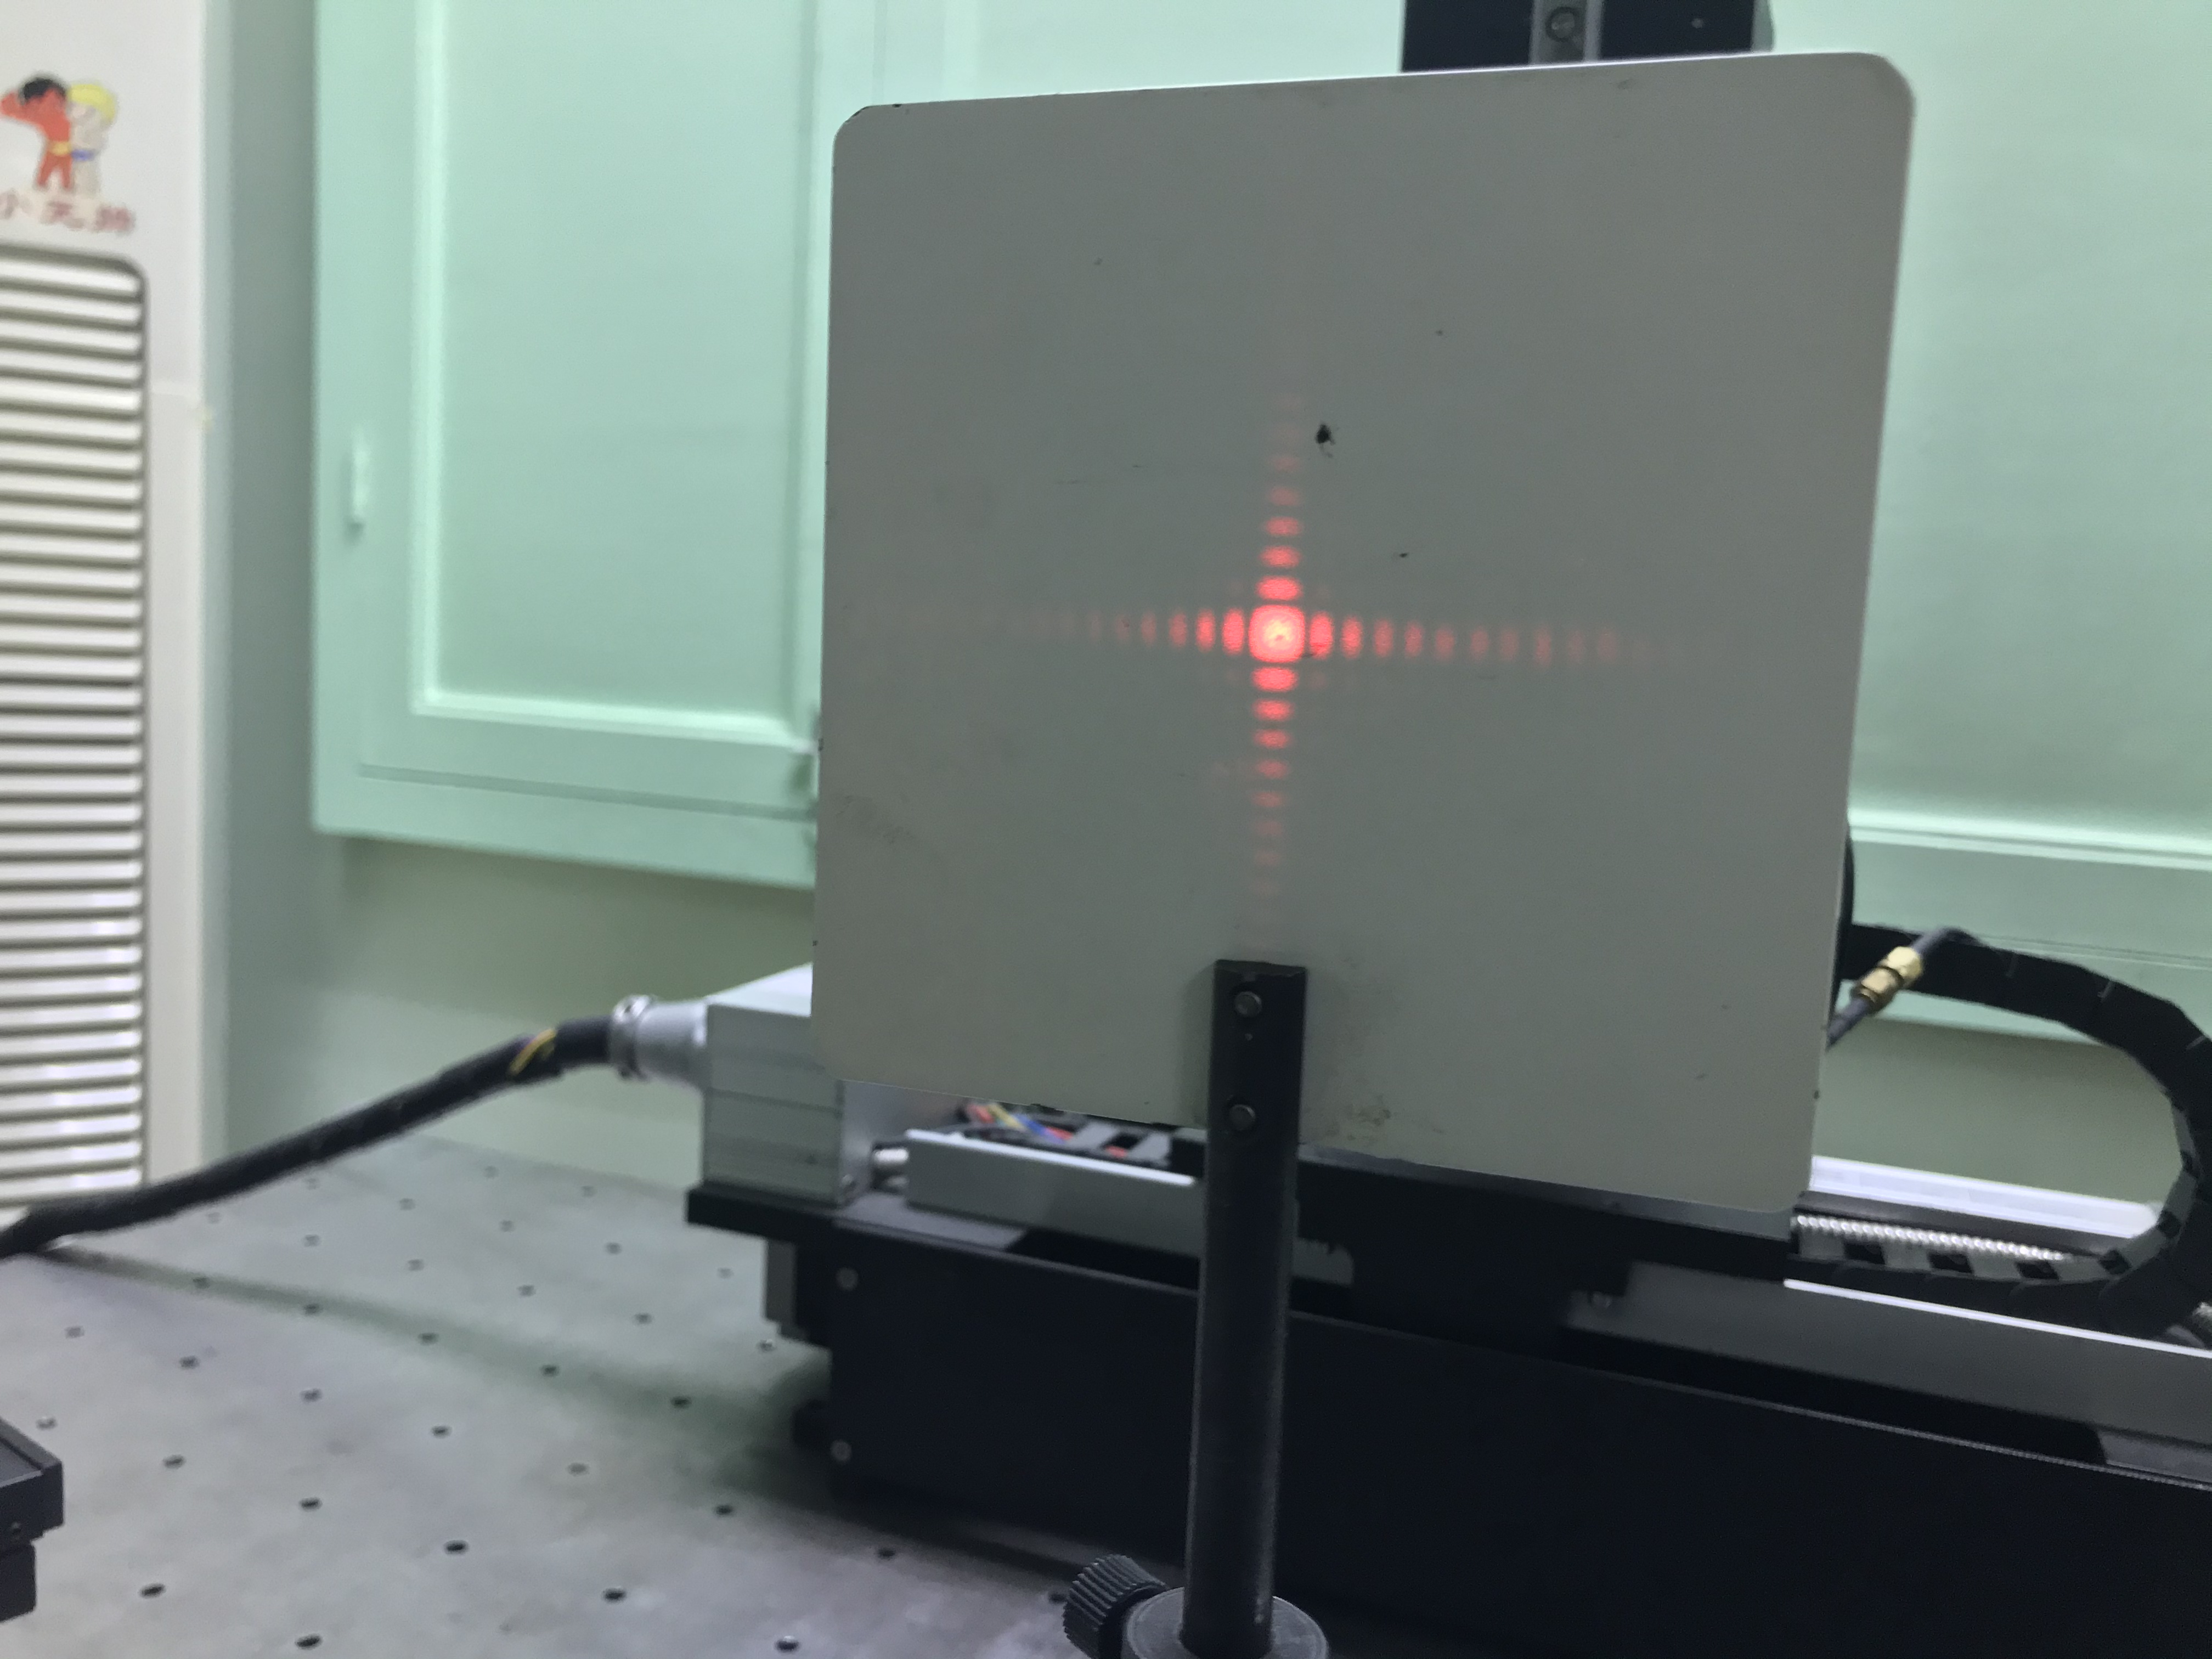
\includegraphics[width=\textwidth]{danfangkong.jpg}
            \caption{单方孔}
        \end{subfigure}  
        \begin{subfigure}[b]{0.45\textwidth}
            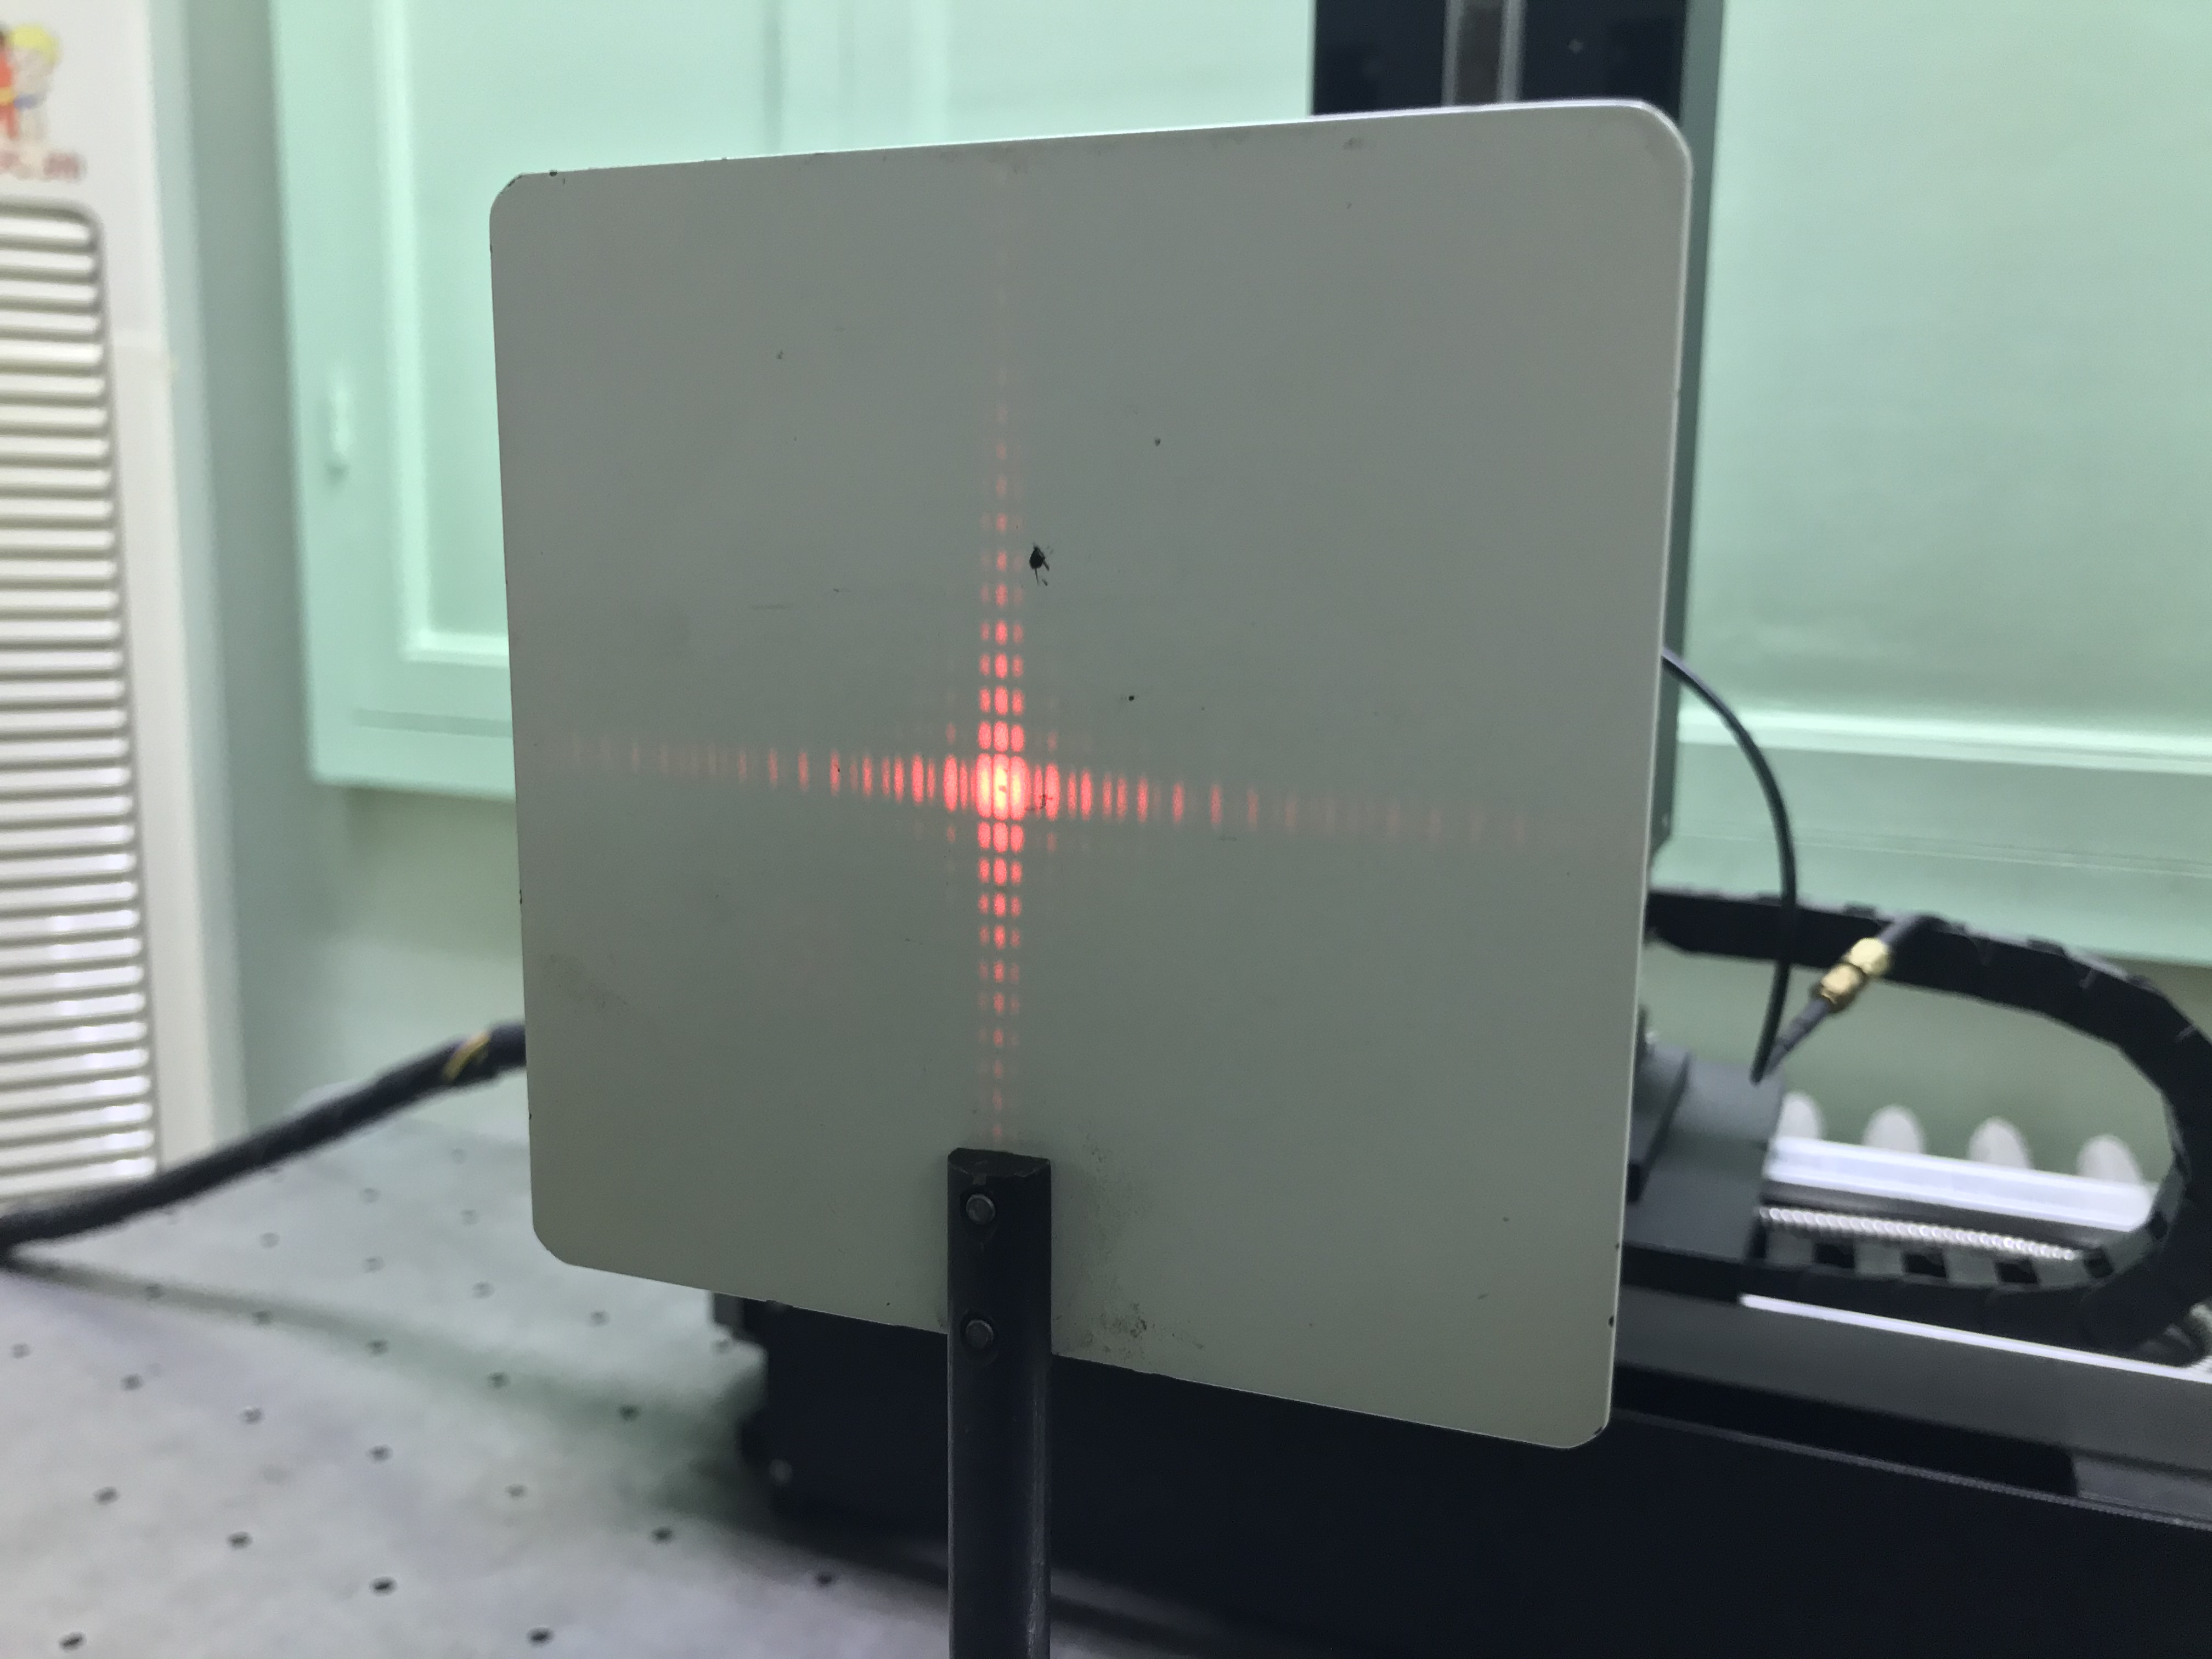
\includegraphics[width=\textwidth]{shuangfangkong.jpg}
            \caption{双方孔}
        \end{subfigure}
        %\vspace{1ex}
        
        \begin{subfigure}[b]{0.45\textwidth}
            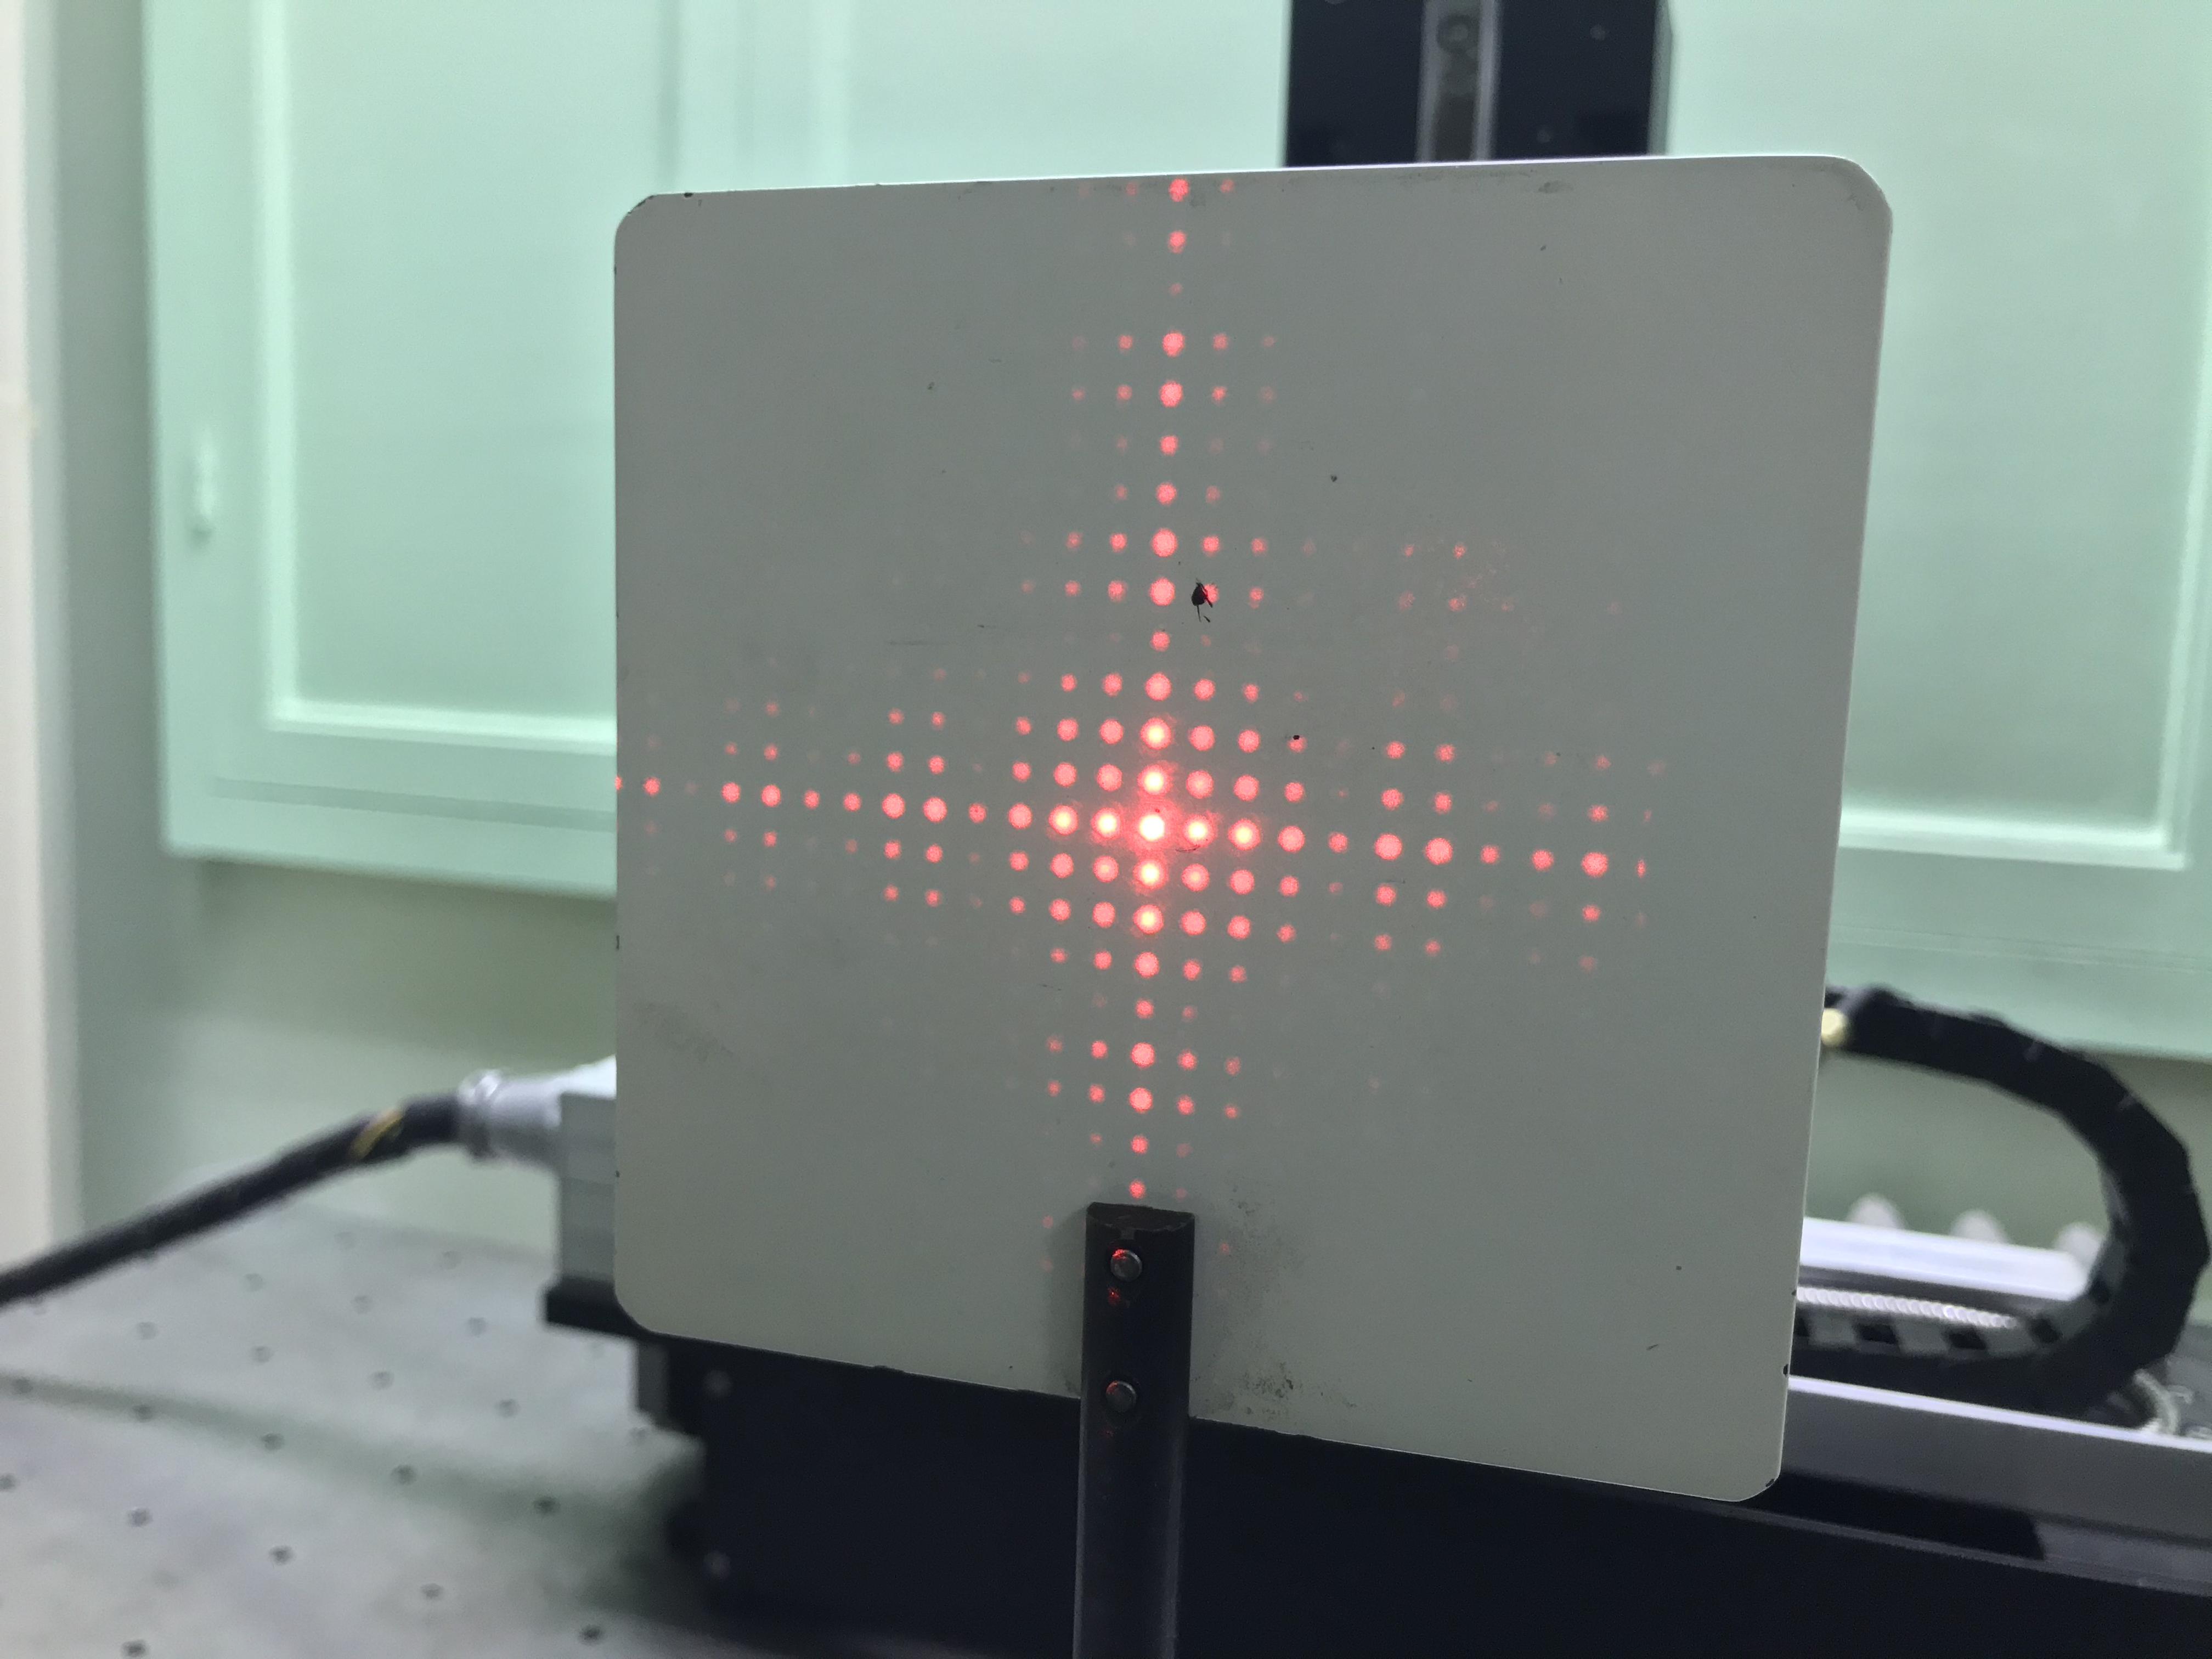
\includegraphics[width=\textwidth]{fangkongfangzhen.jpg}
            \caption{方孔方阵}            
        \end{subfigure}       
        \begin{subfigure}[b]{0.45\textwidth}
            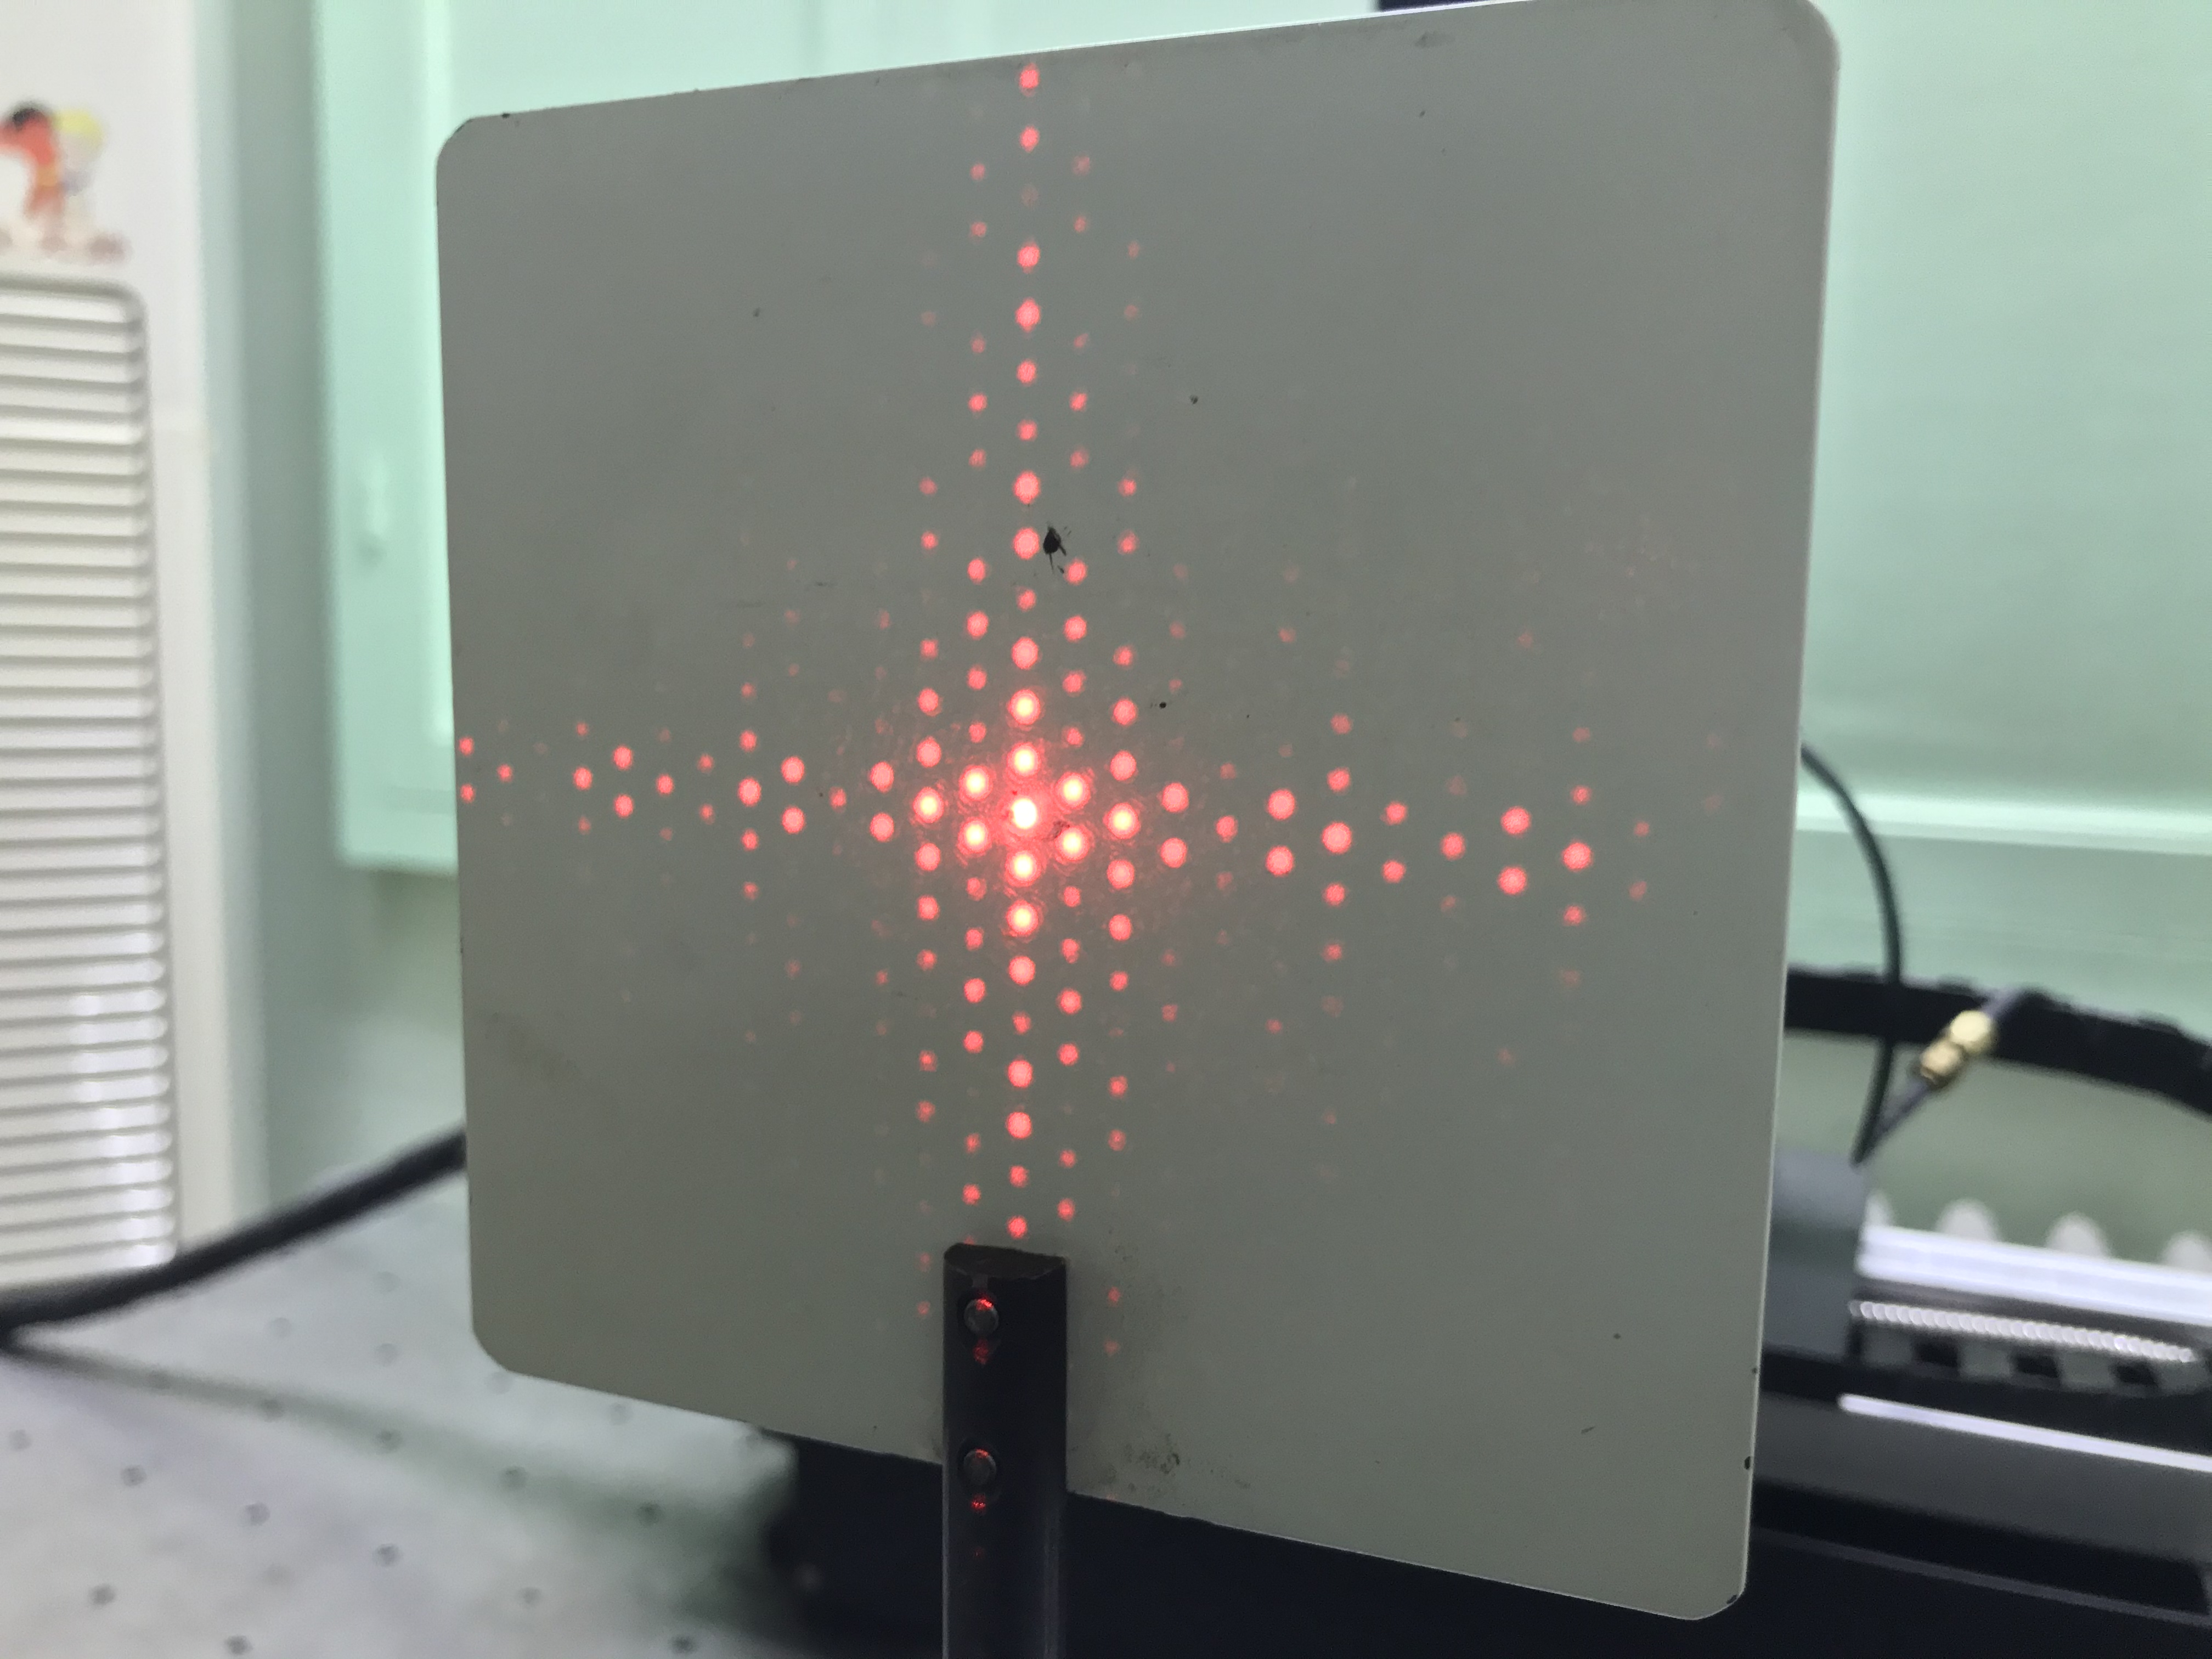
\includegraphics[width=\textwidth]{fangkongmipai.jpg}
            \caption{方孔密排}
        \end{subfigure}
        
        \begin{subfigure}[b]{0.45\textwidth}
            \includegraphics[width=\textwidth]{yuankongfangzhen.jpg}
            \caption{圆孔方阵}
        \end{subfigure}
        \begin{subfigure}[b]{0.45\textwidth}
            \includegraphics[width=\textwidth]{yuankongmipai.jpg}
            \caption{圆孔密排}
        \end{subfigure}
    \end{figure*}
    
    \newpage
    
    \begin{figure*}
        \centering
        \begin{subfigure}[b]{0.45\textwidth}
            \includegraphics[width=\textwidth]{dengbian.jpg}
            \caption{等边三角形}
        \end{subfigure}
        \begin{subfigure}[b]{0.45\textwidth}
            \includegraphics[width=\textwidth]{dengyao.jpg}
            \caption{等腰三角形}    
        \end{subfigure}

        \begin{subfigure}[b]{0.45\textwidth}
            \includegraphics[width=\textwidth]{juxingfangkong.jpg}
            \caption{矩形方孔}
        \end{subfigure}
        \begin{subfigure}[b]{0.45\textwidth}
            \includegraphics[width=\textwidth]{wujiaoxing.jpg}
            \caption{五角星}    
        \end{subfigure}
    \end{figure*}

    \section{分析与讨论}
    
    \subsection{误差分析与不确定度计算}
    \subsubsection{实验中可能的误差来源}
    光路未调整到标准的夫琅和费衍射远场光路可能会带来误差。若衍射屏没有垂直于台面,
    或者条纹没有与探测器移动方向水平,会导致光斑对称性不高,从而导致$\Delta x$的测量
    出现误差。若光没有垂直于衍射屏入射,也会导致主极强和次极强的位置出现误差。

    曲线寻峰和曲线寻谷带来的误差。实验中对于极强点和暗纹的位置是通过对光强曲线寻峰寻谷
    得到的,但曲线在放大后往往是非常曲折的,所以很难找到真正的极大值或极小值点,因而在
    极强点和暗纹位置会出现误差,从而导致$\Delta x$出现误差。

    距离测量的误差。实验中使用钢板尺测量衍射屏到探测器探头的距离,一方面这个距离测定起来
    比较困难,很难标定起点和终点确切位置也很难保证钢板尺平行于光路;另一方面读数过程中也会
    带来误差,这两部分都会导致距离测量,也就是$Z$项的误差。

    \subsubsection{不确定度计算}
    测量$Z$时,在标定衍射屏位置的时候会有$e_1=1cm$左右误差,探测器边缘位置标定起来比较准确,
    基本不会有误差。此外,这两个位置读数时还要考虑刻度尺的允差$e_{2,3}=0.1cm$,故Z的误差:
    $$\sigma_Z=\sqrt{(\frac{e_1}{\sqrt{3}})^2+(\frac{e_2}{\sqrt{3}})^2+(\frac{e_3}{\sqrt{3}})^2}=0.58cm$$

    计算$\Delta x$时,极强或暗纹的位置会有$e_{1,2}0.005mm$的误差,故:
    $$\sigma_{\Delta x}=\sqrt{(\frac{e_1}{2\sqrt{3}})^2+(\frac{e_1}{2\sqrt{3}})^2}=0.002mm$$

    根据缝宽和缝间距的计算公式,可以得出缝宽和缝间距的不确定度:
    $$\frac{\sigma_{b_1}}{b_1}=\sqrt{(\frac{\sigma_{\Delta_x}}{\Delta_x})^2+(\frac{\sigma_Z}{Z})^2},\sigma_{b_1}=1.49\mu m$$
    $$\frac{\sigma_{b_2}}{b_2}=\sqrt{(\frac{\sigma_{\Delta_x}}{\Delta_x})^2+(\frac{\sigma_Z}{Z})^2},\sigma_{b_2}=0.27\mu m$$
    $$\frac{\sigma_{d}}{d}=\sqrt{(\frac{\sigma_{\Delta_x}}{\Delta_x})^2+(\frac{\sigma_Z}{Z})^2},\sigma_{d}=0.63\mu m$$
    
    所以测量结果分别为:
    $$b_1=(178.1\pm1.49)\mu m ,\ b_2=(39.1\pm0.27)\mu m ,\ d = (91.8\pm0.63)\mu m$$

    \subsection{衍射图样和衍射结构之间的关系}
    不同衍射结构基本上均可以看成某种简单的衍射结构的叠加与组合,如圆孔衍射可以看成单缝衍射旋转了$360\degree$,
    矩形孔衍射可以看成正交的两个方向的单缝衍射的叠加和组合。这些衍射结构产生的衍射条纹也可以看成是单缝衍射条纹的叠加与组合。

    衍射结构某一方向上线度越小,相应方向上的衍射条纹就越宽。如矩形孔x方向的“长”大于y方向的“宽”,则
    衍射图样x方向的宽度就比y方向上小。

    另外在多孔、多缝的情况下,除了这些孔、缝各自进行衍射,他们还会发生相互的干涉,使衍射图样进一步呈现明暗交替
    的干涉图样的特点。

    \section{收获与感想}
    本次实验中,在调节光路中用到了之前在测凹透镜焦距实验中用到过的通过光屏移近移远看
    光斑是否在同一位置来判断光路是否水平的方法,可以看出这是光学实验中判断光路情况的常用方法,
    今后可能还会多次用到。

    实验中使用了探测器和计算机软件直接测量并绘制了光强曲线,相较于其他实验中只用到传统仪器,
    计算机和探测器的使用提高了效率,但这也给实验带来的一定的限制条件如必须使衍射条纹和探测器移动方向平行。

    通过这次实验,对单缝、多缝衍射有了一个定量上的认识,同时也观察了不同衍射结构的衍射图样。这些图样都非常漂亮,
    极具物理学美感。
    
\end{document}